\newcommand{\browseUp}{$self.browseUp(nextStep, firstNodeIterator, endNodeIterator)$\xspace}
\newcommand{\browseDown}{$self.browseDown(child, firstNodeIterator, endNodeIterator, self)$\xspace}

\section{Modélisation d'une \dtd}
\begin{figure}[H]
  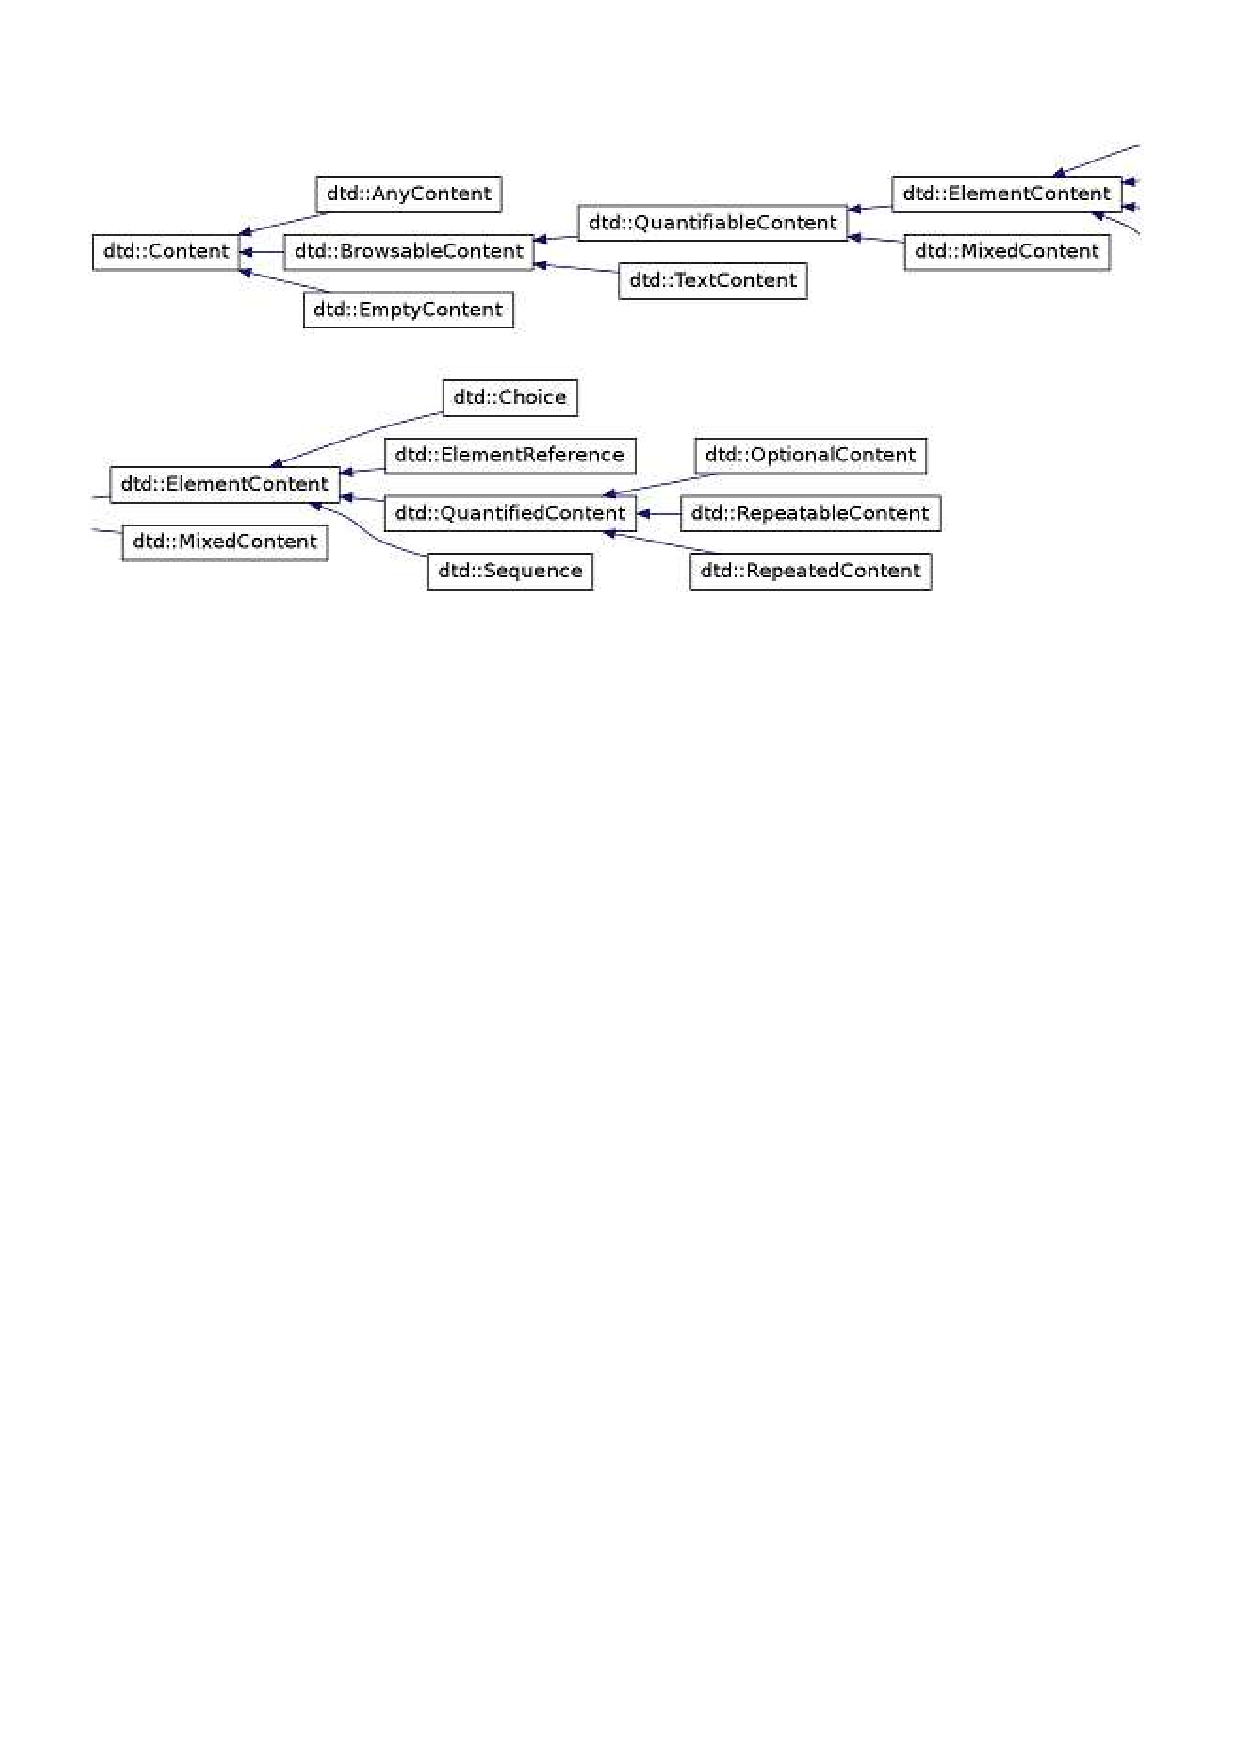
\includegraphics{Structure_DTD_resumee.pdf}
  \caption{Structure compact d'un DTD}
\end{figure}
  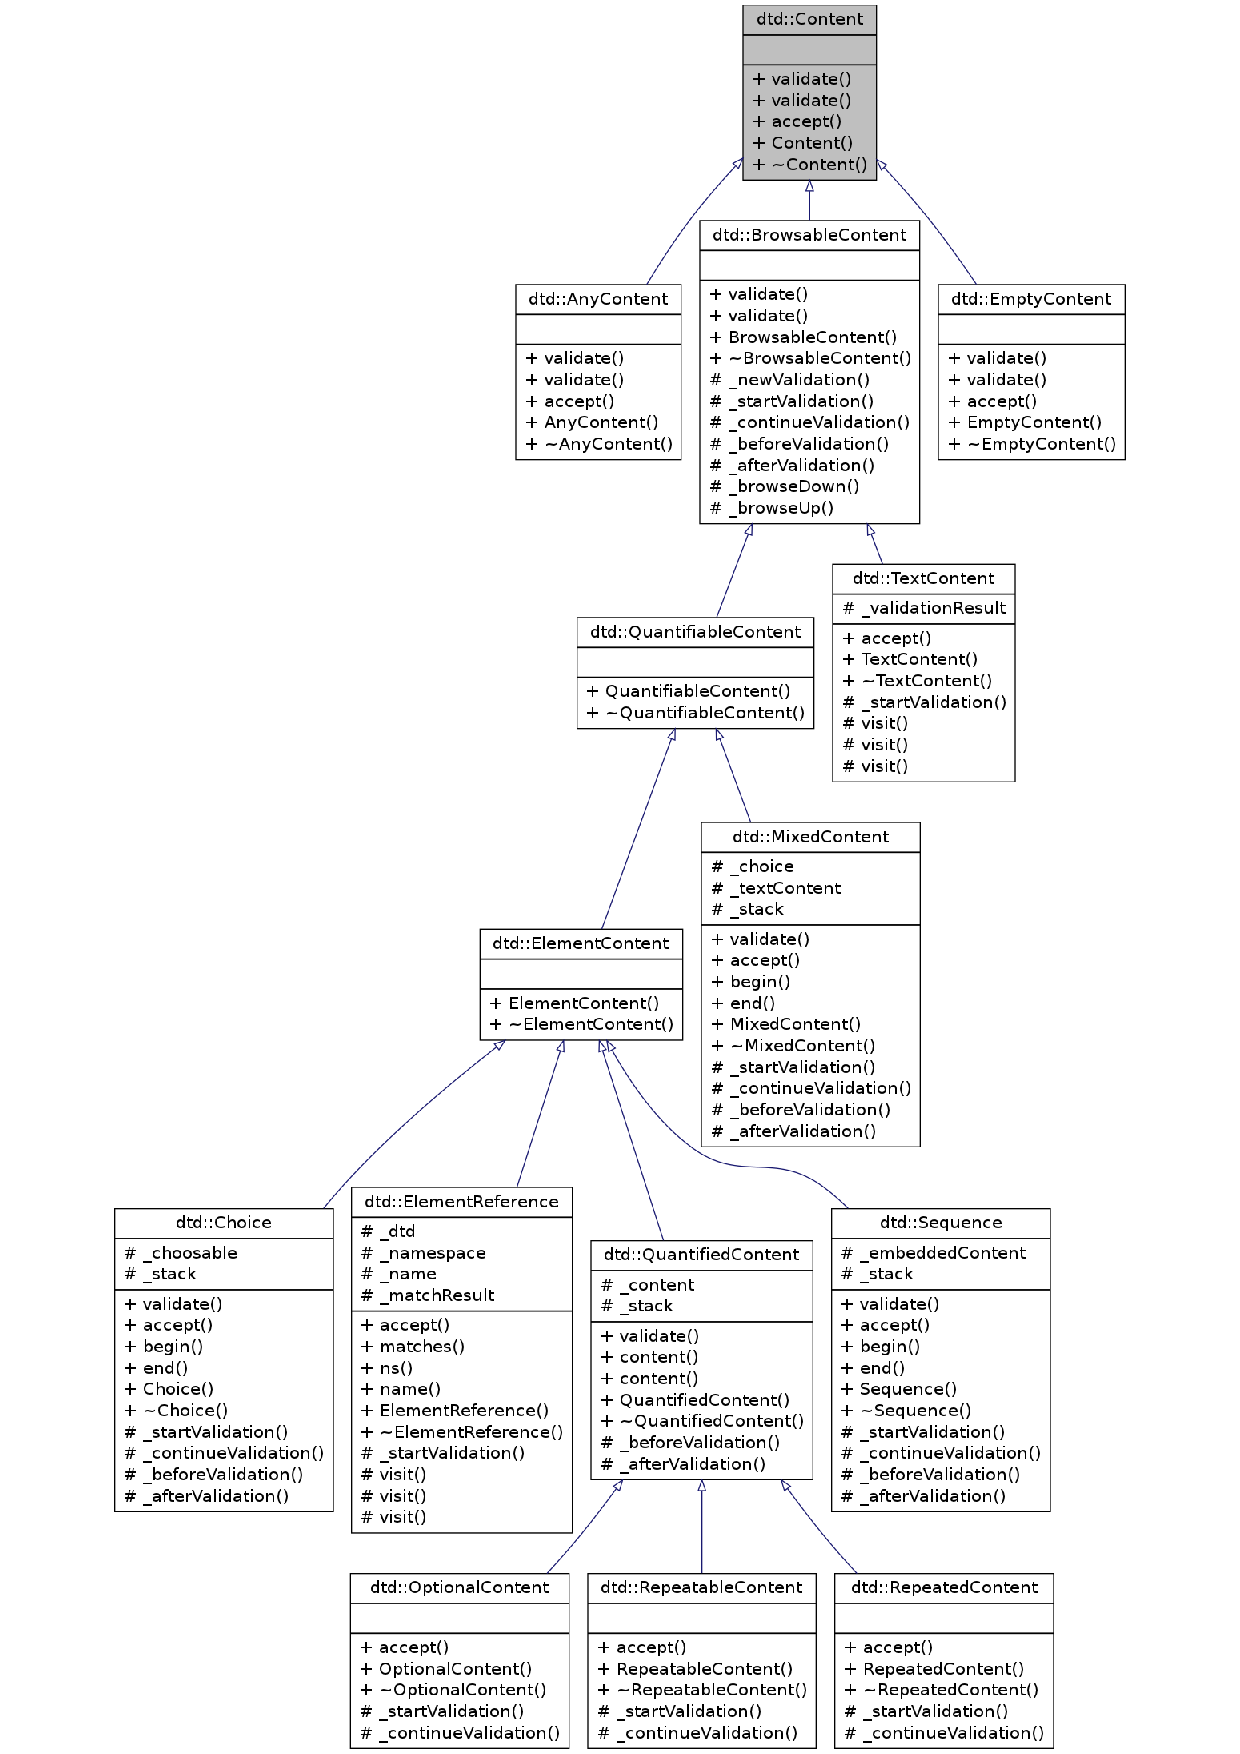
\includegraphics{Structure_DTD_complete.pdf}
\kw{Content} représente le contenu d'un élément dans la \dtd, c'est-à-dire la dernière partie de la balise \kw{<!ELEMENT nom contenu>}. Il permet d'effectuer une validation de la structure d'un noeud \xml. Il définit pour cela une interface simple composée des deux versions de la méthode \kw{validate} ; celle-ci renvoie vrai ou faux en fonction de l'adéquation du contenu du noeud passé en paramètre avec le contenu (classe \kw{Content}) sur lequel a été appelé la méthode. On suppose, lorsque ces méthodes sont appelées, que la version appelée correspond au type réel du noeud.

Parmi les classes dérivées directement de \kw{Content}, on retrouve :
\begin{description}
\item[\kw{EmptyContent}] Contenu vide. Valide n'importe quel noeud de type \kw{MarkupNode}.
\item[\kw{AnyContent}] Contenu quelconque. Valide n'importe quel noeud de type \kw{MarkupNode} ou \kw{CompositeMarkupNode}.
\item[\kw{BrowsableContent}] Contenu plus complexe, potentiellement composite et organisé sous forme d'arbre, et donc navigable pour la validation.
\end{description}

  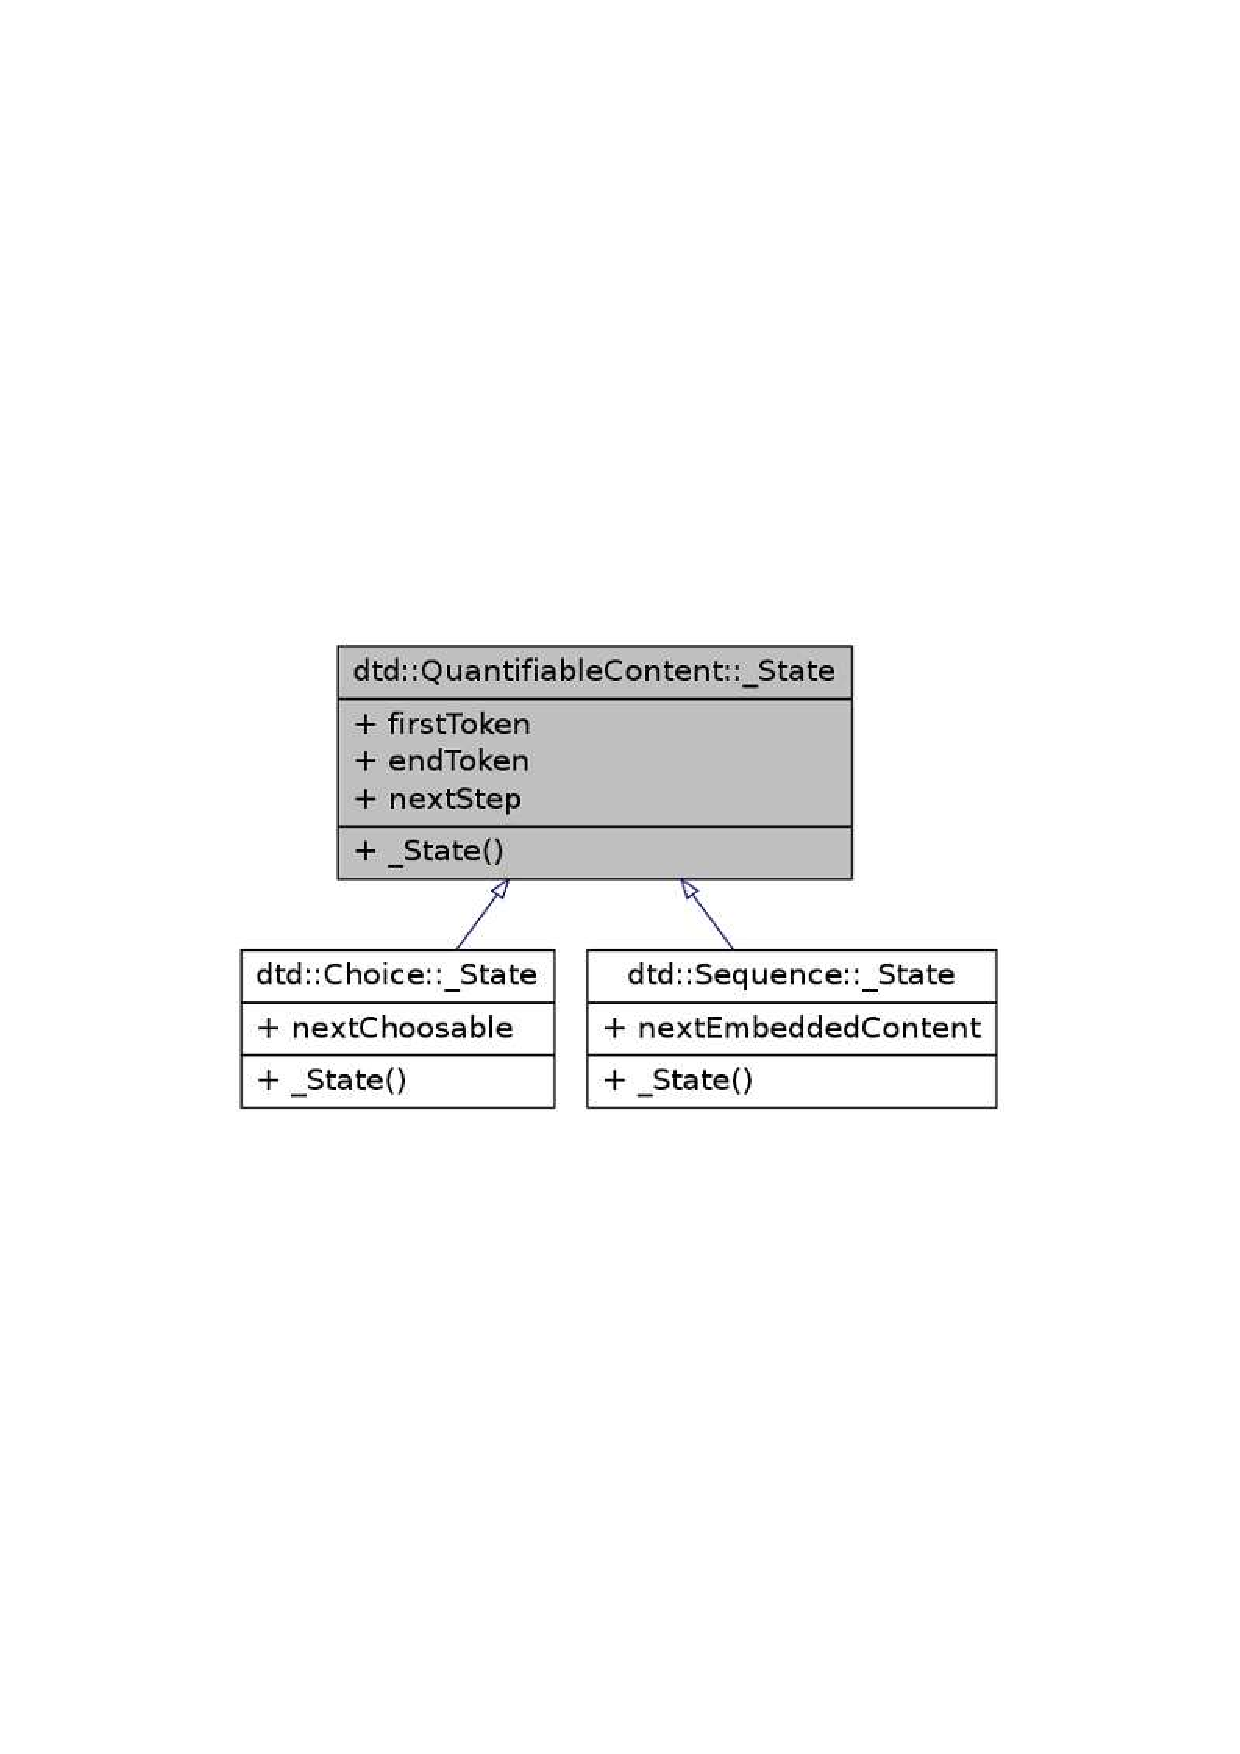
\includegraphics{dtd_quantifiable_content.pdf}
  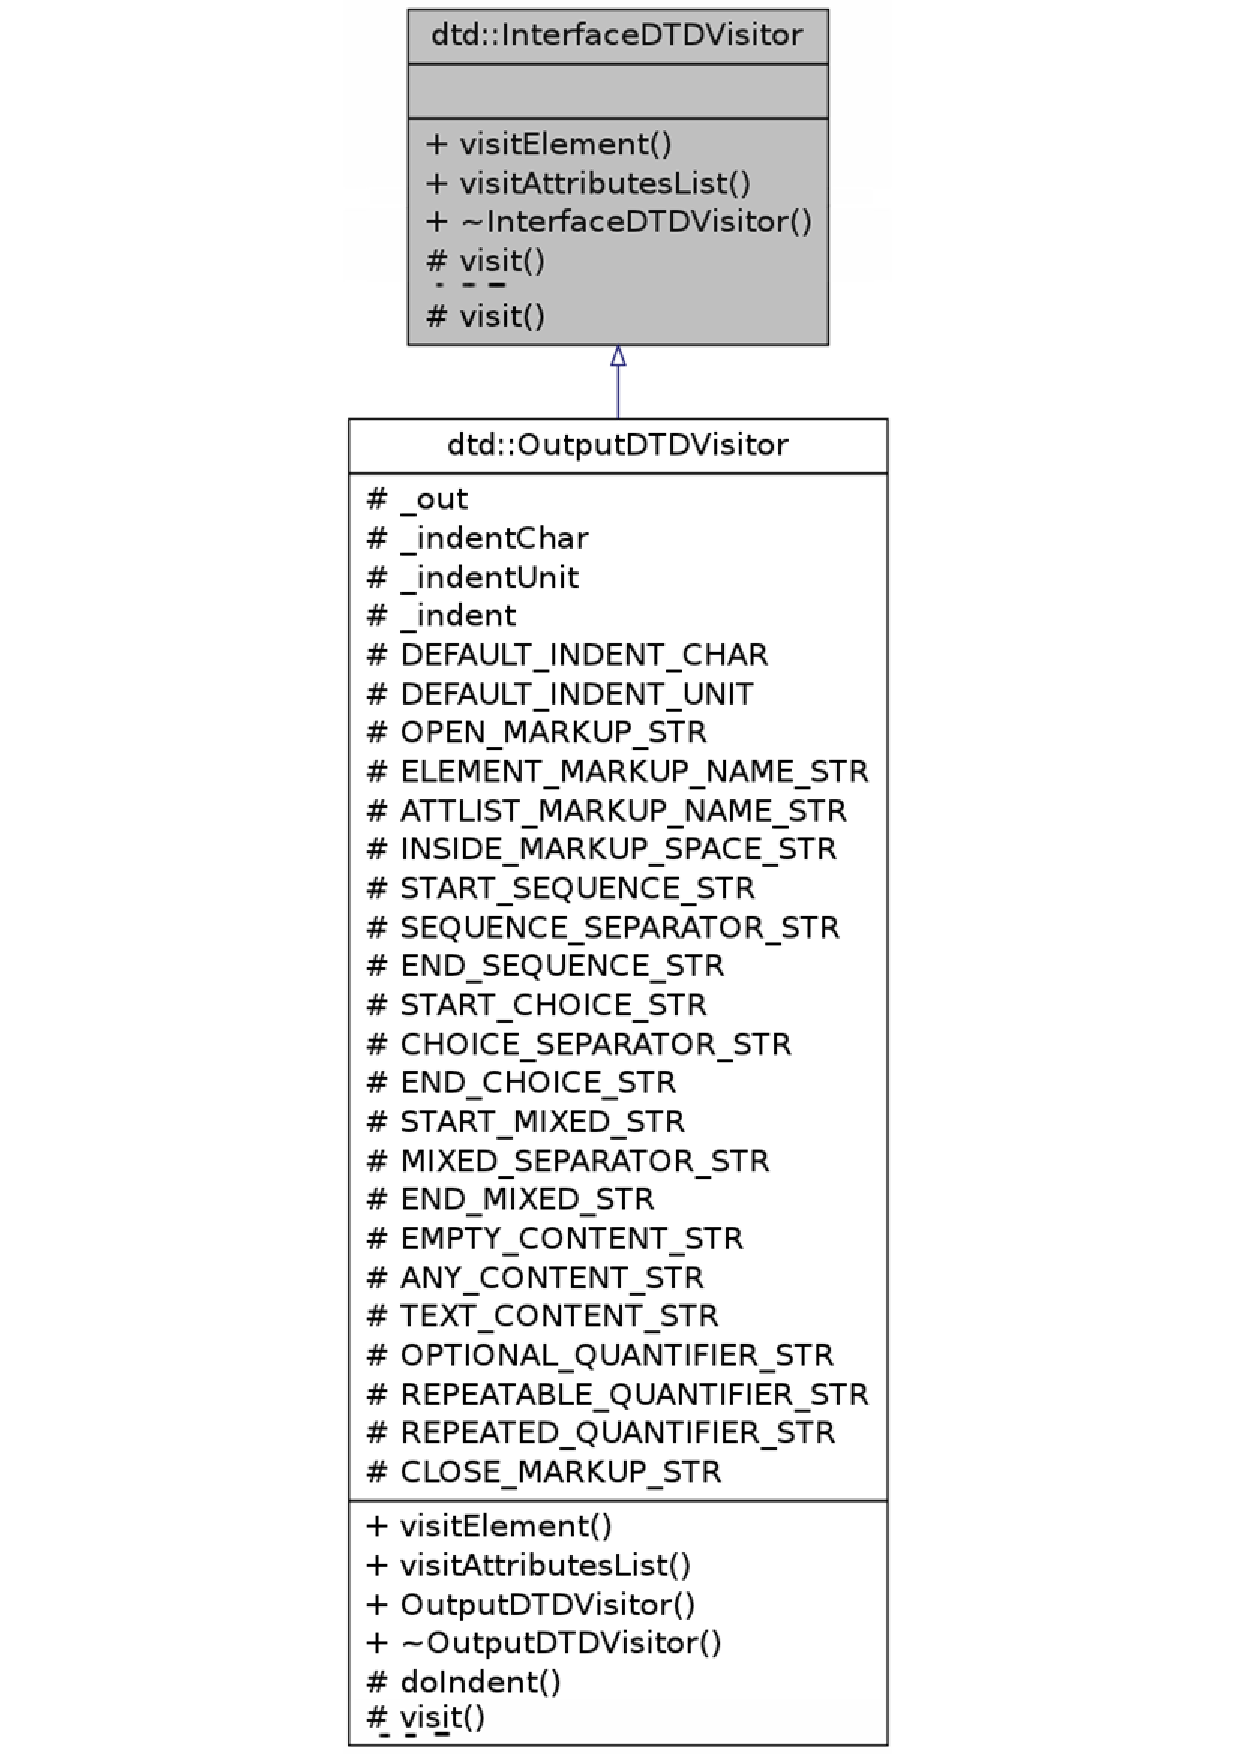
\includegraphics{dtd_visitor.pdf}

\subsection{Validation}
La validation consiste, à partir de la liste des noeuds fils d'un noeud \xml, à leur faire correspondre un arbre de contenu (classe \kw{Content}).

\subsubsection{Algorithme général}
L'algorithme de validation effectue un parcours en profondeur de l'arbre de contenu, avec backtracking. Dans la suite du document, nous étudierons séparément la navigation dans l'arbre, le backtracking et la validation de chaque type particulier de contenu.

\subsubsection{Navigation}
Une validation suit, classiquement, un parcours en profondeur de l'arbre de contenu.

La classe abstraite \kw{BrowsableContent} met en place l'ensemble des méthodes nécessaires à la navigation dans l'arbre de contenu.
En voici une description succinte :
\begin{description}
\item[\kw{+validate(:CompositeMarkupNode):boolean}] Effectue la validation proprement dite (interface client).
\item[\kw{\#newValidation(firstToken:ChildrenIterator, endToken:ChildrenIterator, nextStep:BrowsableContent):boolean}] Méthode protégée appelée sur le contenu suivant lors d'un accès en \og descendant \fg dans l'arbre. Tente de valider (de \og matcher \fg) un maximum de jetons (noeuds enfants) de la liste donnée en paramètre, avec pour contrainte que la validation de la prochaine étape reste d'actualité.
\item[\kw{\#continueValidation(currentToken:ChildrenIterator):boolean}] Méthode protégée appelée sur le contenu suivant lors d'un accès en \og remontant \fg dans l'arbre. Continue la validation entreprise lors du dernier appel à newValidation sur le même objet.
\end{description}

Ainsi, la navigation pourrait être modélisée comme suit :
\begin{algorithm}[H]
\caption{\kw{newValidation}}
\begin{algorithmic}
\REQUIRE $firstNodeIterator$ and $endNodeIterator$, iterators to a list of nodes
\REQUIRE $nextStep$, another BrowsableContent (optional)
\ENSURE True if the node has been validated, false otherwise.
\STATE Perform some validations on the node (potentially incrementing $firstNodeIterator$)
\FORALL{child node $child$}
\STATE Call $child.newValidation(firstNodeIterator, endNodeIterator, self)$
\ENDFOR
\STATE Perform some other validations on the node (potentially incrementing $firstNodeIterator$)
\IF{each validation was successful}
\IF{$nextStep$ is a parameter}
\RETURN $nextStep.continueValidation(firstNodeIterator)$
\ELSE
\IF{$firstNodeIterator$ has reached the end of the list}
\RETURN \TRUE
\ELSE
\RETURN \FALSE
\ENDIF
\ENDIF
\ELSE
\RETURN \FALSE
\ENDIF
\end{algorithmic}
\end{algorithm}

Ce qui correspond aux diagrammes suivants :
\begin{figure}[H]
\caption{Diagramme de séquences d'un exemple de parcours}
\includegraphics[width=\textwidth]{Validation_Parcours_sequence}
\end{figure}
\begin{figure}[H]
\caption{Diagramme de collaboration d'un exemple de parcours}
\includegraphics[width=\textwidth]{Validation_Parcours_collaboration}
\end{figure}

Cependant, les méthodes \kw{newValidation} et \kw{continueValidation} sont protégées, et ne peuvent donc pas être appelées depuis d'autres instances de classes dérivées (en C++, tout au moins). Afin d'accéder à ces méthodes (protégées) depuis d'autres objets de classes dérivées de \kw{BrowsableContent}, il faut définir les méthodes suivantes :
\begin{description}
\item[\kw{\#browseDown(childContent:BrowsableContent, firstToken:ChildrenIterator, endToken:ChildrenIterator, nextStep:BrowsableContent):boolean}] Exécute la descente dans l'arbre de contenu. Consiste à appeler la méthode \kw{newValidation} sur le contenu \kw{childContent}.
\item[\kw{\#browseUp(parentContent:BrowsableContent, currentToken:ChildrenIterator, endToken:ChildrenIterator):boolean}] Exécute la remontée dans l'arbre de contenu. Consiste à appeler la méthode \kw{newValidation} sur le contenu \kw{childContent}. Si l'arbre a été totalement parcouru (nextStep n'existe pas), cette méthode se charge de renvoyer vrai si la liste des enfants a été totalement parcourue, faux sinon.
\end{description}

Ces méthodes sont appelées sur lui-même par un objet désirant continuer la navigation.
On obtient le schéma de navigation suivant :
\begin{algorithm}[H]
\caption{\kw{newValidation}}
\begin{algorithmic}
\REQUIRE $firstNodeIterator$ and $endNodeIterator$, iterators to a list of nodes
\REQUIRE $nextStep$, another BrowsableContent (optional)
\ENSURE True if the node has been validated, false otherwise.
\STATE Perform some validations on the node (potentially incrementing $firstNodeIterator$)
\FORALL{child node $child$}
\STATE Call \browseDown
\ENDFOR
\STATE Perform some other validations on the node (potentially incrementing $firstNodeIterator$)
\IF{each validation was successful}
\RETURN \browseUp
\ELSE
\RETURN \FALSE
\ENDIF
\end{algorithmic}
\end{algorithm}

En réalité, la méthode \kw{newValidation} n'implémente pas directement la validation. Elle se contente d'appeler des patrons de méthodes permettant d'effectuer un pré-traitement, une validation proprement dite, et un post-traitement. Cela permet d'effectuer des empilements d'états nécessaires à l'implémentation des opérateurs de quantification (cf. section \ref{valid_spec}). Les patrons en questions (méthodes virtuelles définies dans les classes dérivées) sont les suivants :
\begin{description}
\item[\kw{\#beforeValidation(firstToken:ChildrenIterator, endToken:ChildrenIterator, nextStep:BrowsableContent):boolean}] Pré-traitement précédant une validation.
\item[\kw{\#startValidation(firstToken:ChildrenIterator, endToken:ChildrenIterator, nextStep:BrowsableContent):boolean}] Première étape d'une validation, potentiellement suivie d'appels à \kw{continueValidation}. C'est cette méthode en particulier qui implémente les spécificités du \og matching \fg de chaque type de contenu.
\item[\kw{\#afterValidation():boolean}] Post-traitement précédant une validation.
\end{description}
%Pour résumer, voici un diagramme de séquences représentant le schéma type d'une navigation ainsi que l'algorithme global :
%\begin{figure}[H]
%\caption{\TODO{Diagramme de séquences BrowsableContent::validate}}
%\end{figure}
%\begin{algorithm}[H]
%\caption{\TODO{Algorithme récapitulatif}}
%\end{algorithm}

\subsubsection{Backtracking}
Etant donnée la manière dont l'arbre est parcouru, chaque noeud effectuant un choix (\kw{Choice}, \kw{QuantifiedContent}, \kw{MixedContent}) est mis au courant si la suite de la validation n'a pas pu se faire. Il est donc possible, au niveau de chacun de ces noeuds, de gérer le backtracking :
\begin{itemize}
\item après un \kw{Choice} ou un \kw{MixedContent}, si la suite de la validation n'a pas pu être effectuée, on essaye le choix suivant. Si on a atteint la fin de la liste, on renvoie faux pour signaler au contenu parent qu'il faut effectuer un backtracking.
\item après un \kw{QuantifiedContent}, si la suite de la validation n'a pas pu être effectuée, on tente de \og matcher \fg un jeton de moins, puis de relancer la suite de la validation. Si on arrive en dessous du nombre minimum de \og matching \fg, on renvoie faux pour signaler au contenu parent qu'il faut effectuer un backtracking.
\end{itemize}

\subsubsection{Validation spécifique}
\label{valid_spec}
Ici sont décrites les spécificités de la validation de chaque type de contenu, donc les différentes implémentations de \kw{startValidation}, et s'il y a lieu de \kw{continueValidation}.

\begin{algorithm}[H]
\caption{\kw{TextContent::startValidation}}
\begin{algorithmic}
\REQUIRE $firstNodeIterator$ and $endNodeIterator$, iterators to a list of nodes
\REQUIRE $nextStep$, another BrowsableContent (optional)
\ENSURE True if the node has been validated, false otherwise.
\IF{node pointed by $firstNodeIterator$ is an instance of $TextNode$}
\RETURN \browseUp
\ELSE
\RETURN \FALSE
\ENDIF
\end{algorithmic}
\end{algorithm}

\begin{algorithm}[H]
\caption{\kw{ElementReference::startValidation}}
\begin{algorithmic}
\REQUIRE $firstNodeIterator$ and $endNodeIterator$, iterators to a list of nodes
\REQUIRE $nextStep$, another BrowsableContent (optional)
\ENSURE True if the node has been validated, false otherwise.
\IF{node pointed by $firstNodeIterator$ is an instance of $TextNode$}
\RETURN \FALSE
\ELSE
\IF{namespace and name of $firstNodeIterator$ match with this object's ones}
\RETURN \browseUp
\ELSE
\RETURN \FALSE
\ENDIF
\ENDIF
\end{algorithmic}
\end{algorithm}

\begin{algorithm}[H]
\caption{\kw{Choice::startValidation}}
\begin{algorithmic}
\REQUIRE $firstNodeIterator$ and $endNodeIterator$, iterators to a list of nodes
\REQUIRE $nextStep$, another BrowsableContent (optional)
\ENSURE True if the node has been validated, false otherwise.
\WHILE{end of child list has not been reached \AND no matching has been found among childs}
\STATE \browseDown
\ENDWHILE
\IF{a matching has been found}
\RETURN \TRUE
\ELSE
\RETURN \FALSE
\ENDIF
\end{algorithmic}
\end{algorithm}

\begin{algorithm}[H]
\caption{\kw{Choice::continueValidation}}
\begin{algorithmic}
\REQUIRE $currentNodeIterator$, iterator to a list of nodes
\ENSURE True if the node has been validated, false otherwise.
\STATE Load $endNodeIterator$ (has to be stored in $beforeValidation$ procedure)
\STATE Load $nextStep$ (has to be stored in $beforeValidation$ procedure)
\RETURN \browseUp
\end{algorithmic}
\end{algorithm}

\begin{algorithm}[H]
\caption{\kw{MixedContent::startValidation}}
\begin{algorithmic}
\REQUIRE $firstNodeIterator$ and $endNodeIterator$, iterators to a list of nodes
\REQUIRE $nextStep$, another BrowsableContent (optional)
\ENSURE True if the node has been validated, false otherwise.
\IF{node pointed by $firstNodeIterator$ is an instance of $TextNode$ \AND \browseUp}
	\RETURN \TRUE
\ELSE
	\WHILE{end of child list has not been reached \AND no matching has been found among childs}
		\STATE \browseDown
	\ENDWHILE
	\IF{a matching has been found}
		\RETURN \TRUE
	\ELSE
		\RETURN \FALSE
	\ENDIF
\ENDIF
\end{algorithmic}
\end{algorithm}

\begin{algorithm}[H]
\caption{\kw{MixedContent::continueValidation}}
\begin{algorithmic}
\REQUIRE $currentNodeIterator$, iterator to a list of nodes
\ENSURE True if the node has been validated, false otherwise.
\STATE Load $endNodeIterator$ (has to be stored in $beforeValidation$ procedure)
\STATE Load $nextStep$ (has to be stored in $beforeValidation$ procedure)
\RETURN \browseUp
\end{algorithmic}
\end{algorithm}

\begin{algorithm}[H]
\caption{\kw{Sequence::startValidation}}
\begin{algorithmic}
\REQUIRE $firstNodeIterator$ and $endNodeIterator$, iterators to a list of nodes
\REQUIRE $nextStep$, another BrowsableContent (optional)
\STATE \COMMENT{The $startValidation$ procedure is not different from this one.}
\RETURN $self.continueValidation(firstNodeIterator$ 
\end{algorithmic}
\end{algorithm}

\begin{algorithm}[H]
\caption{\kw{Sequence::continueValidation}}
\begin{algorithmic}
\REQUIRE $currentNodeIterator$, iterator to a list of nodes
\ENSURE True if the node has been validated, false otherwise.
\STATE Load $endNodeIterator$ (has to be stored in $beforeValidation$ procedure)
\STATE Load $nextStep$ (has to be stored in $beforeValidation$ procedure)
\STATE Load current $child$ (has to be stored in $beforeValidation$ procedure)
\IF{The last child has not been reached}
\STATE \COMMENT{We should match each single child}
\RETURN \browseDown
\ELSE
\STATE \COMMENT{We matched all childs. The result is up to the next step.}
\RETURN \browseUp
\ENDIF
\end{algorithmic}
\end{algorithm}

\begin{algorithm}[H]
\caption{\kw{OptionalContent::startValidation}}
\begin{algorithmic}
\REQUIRE $firstNodeIterator$ and $endNodeIterator$, iterators to a list of nodes
\REQUIRE $nextStep$, another BrowsableContent (optional)
\IF{\browseDown}
\STATE \COMMENT{We first try to include the child in the matching pattern.}
\RETURN \TRUE
\ELSIF{\browseUp}
\STATE \COMMENT{We couldn't include the child in the matching pattern. We try without it.}
\RETURN \TRUE
\ELSE
\STATE \COMMENT{It's definitely not possible to match in these conditions. Try backtracking.}
\RETURN \FALSE
\ENDIF
\end{algorithmic}
\end{algorithm}

\begin{algorithm}[H]
\caption{\kw{OptionalContent::continueValidation}}
\begin{algorithmic}
\REQUIRE $currentNodeIterator$, iterator to a list of nodes
\ENSURE True if the node has been validated, false otherwise.
\STATE Load $endNodeIterator$ (has to be stored in $beforeValidation$ procedure)
\STATE Load $nextStep$ (has to be stored in $beforeValidation$ procedure)
\RETURN \browseUp
\end{algorithmic}
\end{algorithm}

\begin{algorithm}[H]
\caption{\kw{RepeateableContent::startValidation}}
\begin{algorithmic}
\REQUIRE $firstNodeIterator$ and $endNodeIterator$, iterators to a list of nodes
\REQUIRE $nextStep$, another BrowsableContent (optional)
\STATE \COMMENT{The $startValidation$ procedure is not different from this one.}
\RETURN $self.continueValidation(firstNodeIterator$ 
\end{algorithmic}
\end{algorithm}

\begin{algorithm}[H]
\caption{\kw{RepeateableContent::continueValidation}}
\begin{algorithmic}
\REQUIRE $currentNodeIterator$, iterator to a list of nodes
\ENSURE True if the node has been validated, false otherwise.
\STATE Load $endNodeIterator$ (has to be stored in $beforeValidation$ procedure)
\STATE Load $nextStep$ (has to be stored in $beforeValidation$ procedure)
\IF{\browseDown}
\STATE \COMMENT{We first try to include the child in the matching pattern.}
\RETURN \TRUE
\ELSIF{\browseUp}
\STATE \COMMENT{We couldn't include the child in the matching pattern. We try without it.}
\RETURN \TRUE
\ELSE
\STATE \COMMENT{It's definitely not possible to match in these conditions. Try backtracking.}
\RETURN \FALSE
\ENDIF
\end{algorithmic}
\end{algorithm}

\begin{algorithm}[H]
\caption{\kw{RepeatedContent::startValidation}}
\begin{algorithmic}
\REQUIRE $firstNodeIterator$ and $endNodeIterator$, iterators to a list of nodes
\REQUIRE $nextStep$, another BrowsableContent (optional)
\STATE \COMMENT{The child has to be matched at least once}
\RETURN \browseDown
\end{algorithmic}
\end{algorithm}

\begin{algorithm}[H]
\caption{\kw{RepeatedContent::continueValidation}}
\begin{algorithmic}
\REQUIRE $currentNodeIterator$, iterator to a list of nodes
\ENSURE True if the node has been validated, false otherwise.
\STATE Load $endNodeIterator$ (has to be stored in $beforeValidation$ procedure)
\STATE Load $nextStep$ (has to be stored in $beforeValidation$ procedure)
\IF{\browseDown}
\STATE \COMMENT{We first try to include the child in the matching pattern.}
\RETURN \TRUE
\ELSIF{\browseUp}
\STATE \COMMENT{We couldn't include the child in the matching pattern. We try without it.}
\RETURN \TRUE
\ELSE
\STATE \COMMENT{It's definitely not possible to match in these conditions. Try backtracking.}
\RETURN \FALSE
\ENDIF
\end{algorithmic}
\end{algorithm}
